\documentclass[11pt]{article}
\usepackage[margin  = 1in]{geometry}
\usepackage{hyperref}
\bibliographystyle{ieeetr}
\usepackage{amsmath} 
\usepackage{graphicx}
\usepackage{float}
\usepackage{subcaption}
\bibliographystyle{ieeetr}

\begin{document}

\title{Optimizing Terahertz Leaky Wave Antennas Using Deep Learning Predicted Periodically  Modulated Slots}
\author{J. Neronha, H. Guerboukha, and D. Mittleman \\ \\ \small School of Engineering, Brown University, Providence, RI 02912}
\date{}

\maketitle

\section*{Introduction}

The predictive power of neural networks and machine learning techniques more generally have been applied to a vast array problems ever since the neural network was proposed as a computational technique loosely modeling the brain in the mid-twentieth century. \cite{McCulloch:1943vq} This, of course, includes communications technology -- neural networks have been used extensively in the field because of their unique ability to approximate accurate solutions to nonlinear problems that are commonplace in antenna design. Machine learning models are particularly useful in situations where an analytical solution cannot be obtained and/or numerical simulations are expensive \cite{Kim, Massa}. These types of problems are usually split into two cases, forward and inverse problems. The former refers to situations where models attempt to generate the electromagnetic response given some parametric input, while the latter attempts the reverse: predicting those parameters given some signal \cite{9395365}. \\

\noindent Examples of direct problems include approximating an antenna's output given a geometry \cite{8608745} or modeling a metasurface \cite{Nadell:19}, which could take a finite-element model hours or longer to solve, limiting real-time simulation and design. Inverse problem considers the opposite direction, for example reconstructing an image from scattered light \cite{Sun:18}. There have been many applications of neural networks to communications-related problems, for example, in the optimization of massive multiple-input multiple-output (MIMO) systems to improve signal reconstruction quality \cite{8322184} or physical layer design \cite{DBLP:journals/corr/OSheaEC17}. \emph{MORE EXAMPLES HERE?} \\

\noindent We are particularly interested in the inverse problem of terahertz leaky-wave antenna (LWA) design because of its high applicability to the field of communications -- given some arbitrarily desired far-field pattern, how can we quickly design, fabricate, and test an antenna that meets our needs? Periodic leaky wave-antennas are especially interesting for signal design because of their characteristic emissions at various angles, both forward and backwards scattering, that depend on the periodicity, allowing for a wide variety of potential peak angles \cite{6556051}. And while traditional communications systems demand broad angular emission, the terahertz range (i.e. $>$ 100 GHz) requires focusing power along narrow directional beams due to substantial power loss as a result of free path losses at higher frequencies \cite{doi:10.1063/1.5014037, Ghasempour:2020tz}, meaning that highly specific peak profile design is crucial. \\

\noindent LWAs are simple metallic waveguides that have proven very effective in the terahertz range and are particularly interesting because they emit radiation at a frequency-dependent angle with a one-to-one relationship between frequency and angle, which is quite valuable given the narrow character of beams in the terahertz range. \cite{doi:10.1063/5.0033126} They have been used in a number of diverse applications including link discovery \cite{Ghasempour:2020tz}, multiplexing and demultiplexing \cite{Karl:2015uh, Ma:2017vo}, and for radar and object detection purposes \cite{Amarasinghe:20, Amarasinghe:21}. Leaky-wave antennas also stand out for our purposes of rapid design and experimentation because of the ease of fabricating them using hot-stamping techniques \cite{Guerboukha:21}. This inverse problem has been explored in the terahertz range using deep neural networks in the context of designing structures to obtain an optimized geometry that produces the desired signal, particularly in relation to metasurface design \cite{Deng:21, 9602997}. The inverse Leaky-wave antenna problem has also been explored, but using a genetic algorithm and outside of the terahertz range at much higher frequencies \cite{Jafar-Zanjani:2018vy}. \\

\noindent As a result, in this paper, we propose a model to predict the ideal LWA geometry that will generate desired far-field radiation in the terahertz range. Specifically, we suggest an antenna design where a LWA is broken into sub-slots, each of which can either be metallic, transparent, or somewhere in between (i.e. partially transparent). Thus, we find that any slot composed of an array of these sub-slots forms a linear superpositioning of periodic modes that can be used to generate highly specific peak profiles.

\section*{Methodology}

We train a model to predict the slot geometry of the LWA for a desired far-field pattern. We consider a LWA based on a parallel plate waveguide, the fundamental transverse electric (TE$_1$) mode, and a frequency of 200 GHz. Instead of a uniform 1D slot \cite{doi:10.1063/5.0033126}, we discretize the slot into 36 0.5-mm sub-slots that can be transparent, metallic, or somewhere in between (i.e. semi-transparent). This approach is similar to the approach taken in past explorations of metasurface design \cite{Liu:2022tg, Jafar-Zanjani:2018vy}. According to Floquet theory \cite{6556051}, a periodic array of slots excites an infinite number of space harmonics each with its distinct dispersion constant $\beta_p$:

\[\beta=\sqrt{k_0^2 - (\frac{\pi}{h})^2} +\frac{2\pi p}{\Lambda} \tag{1} \label{eq:special}\] 

\noindent where $k_0$ is the wave number, $h$ is the height of the waveguide, and $\Lambda$ is the slot periodicity. These different modes peak at different angles defined by $\cos(\theta)=\beta_p/k_0$, given that the excited modes can be consider fast-wave (i.e., $|\beta_p|>k_0$). Our primary objective is to generate multiple beams with specific magnitudes at specific locations. Therefore, instead of a periodic geometry, we consider a non-periodic array of slots. By Fourier decomposition, we note that any non-periodic slot design can be viewed as a linear combination of periodic designs $\beta_p$, each peaking at an angle $\cos(\theta)=\beta_p/k_0$. The strength (amplitude) of individual peaks can be related to the Fourier coefficients of this decomposition. \\

\noindent Our discretized geometry imposes limits on the possible excited Floquet modes, by constraining the values of $\Lambda$. Indeed, due to the discretization, the possible $\Lambda$ are given by $\Lambda=$. Furthermore, due to the fast-wave requirement (i.e., $|\beta_p|>k_0$), only a few select modes will be able to leak out of the waveguide. We propose two different schemes for generating a desired signal:

\begin{enumerate}
	\item each sub-slot can be either transparent or metallic (left panel of Figure 1)
	\item each sub-slot can also take some intermediate value of opacity (right panel of Figure 1)
\end{enumerate}  

\noindent A schematic of both schemes is shown in Figure 1 below. Additionally, Figure 2 shows all possible peaks from the various modes and periodicities Floquet theory and these peaks overlaid a sample far-field signal from a similar geometry.

\begin{figure}
		\centering
		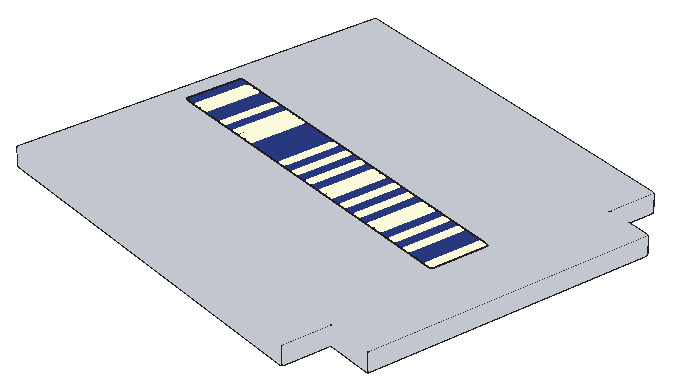
\includegraphics[width = 6in]{figures/fig5.eps}
		\caption{The leaky wave antenna geometry. The left panel shows the binary case, where dark-colored sub-slots represent transparent areas while light colors indicate metallic boundaries. In the right panel, the boundary conditions are no longer discretized and can take on some intermediate value of transparency, as seen by the sub-slots with colors between light and dark.}
\end{figure}


\begin{figure}[H]
	\centering
	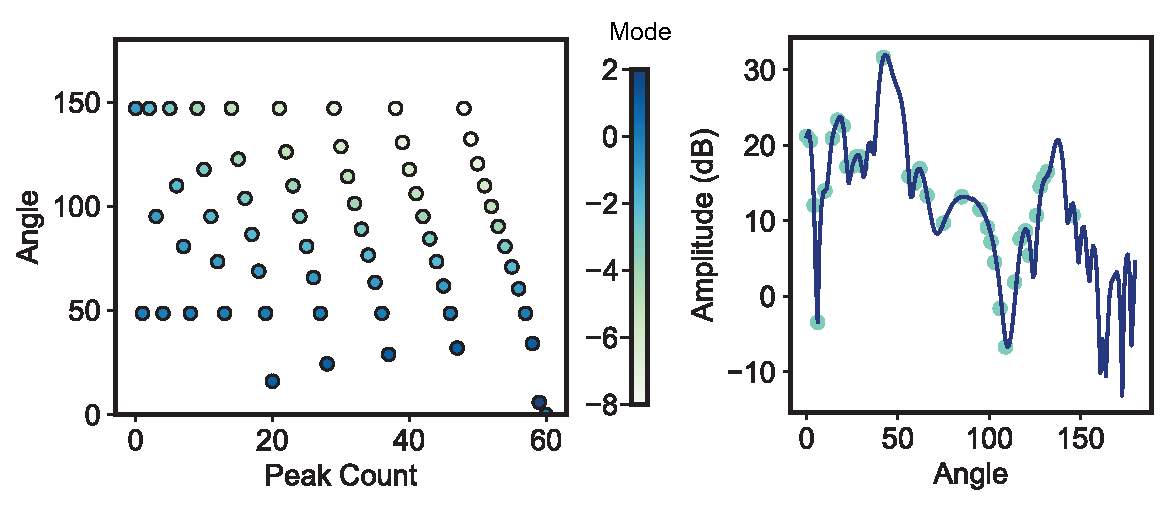
\includegraphics[width=6in]{figures/fig4_labeled2.eps}
	\caption{The left panel shows the possible Floquet modes from any linear combination of modes predicted by Equation 1; as expected, the positive modes occur in forward scattering (< 90$\deg$) and the negative modes in back-scattering. The right panel shows these predicted Floquet modes overlaid on a sample peak profile generated in COMSOL.}
\end{figure}


\noindent To generate our training data, we build a model of a leaky-wave antenna in COMSOL Multiphysics with a slot of length 18 mm divided into 36 sub-slots, each of which is 500 microns in length. 18 sub-slots (exactly half) of the slots are randomly chosen as to be transparent (i.e. a scattering boundary layer) whereas the balance remain metallic and thus do not leak radiation. A similar process is carried out for the grey scheme, except that slots are randomly assigned to buckets of various levels of transparency. We automate this random geometry generation and simulation using MPh \cite{john_hennig_2022_6312347}, an open-source Python package that enables controlling COMSOL via its API. Basic combinatorics theory tells us that there are over 9 billion possible slot designs that can be generated, indicating the usefulness of deep neural networks in this prediction task given the sheer number of possible outputs; using only a few tens of thousands sets of training data, we can predict an optimal slot design for an arbitrary peak profile. \\

\noindent 20,000 instances of COMSOL simulation data is generated as the data source for our deep neural network, with a test-train split of 80-20 \cite{molecules26041111}. A different network and set of training data is used to generate predictions for each sub-slot scheme. Figure 3b above shows the possible values for each peak, giving an approximate range over which we can design peak profiles for this particular geometry. The network, which is built with TensorFlow \cite{tensorflow2015-whitepaper}, a popular deep-learning library, has one convolutional layer for feature extraction connected to six sequential fully-connected layers, each of which have 2000 neurons and use a LeakyReLU activation function with $\alpha = 0.1$. The model uses the Adam optimizer and has a learning rate of 0.0001 and predicts the output of each individual sub-slot with a sigmoid activation function indicating the probability that a given sub-slot should be transparent. The model architecture is visualized in Figure 3. \\

\begin{figure}[H]
	\centering
	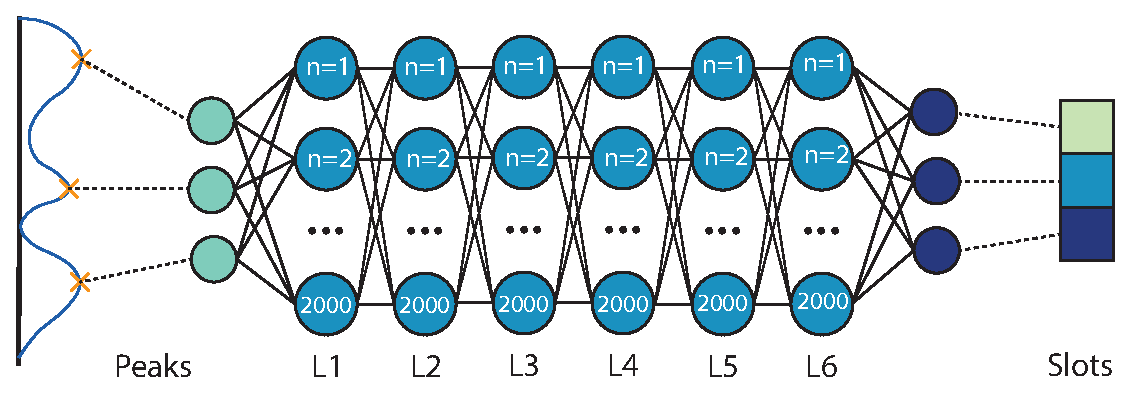
\includegraphics[width=6in]{figures/fig1.eps}
	\caption{Neural network architecture schematic; peaks are used as the input data and passed through six hidden layers to predict the ideal slot design that will yield the closest possible signal.}
\end{figure}

\noindent The tricky part of the inverse problem, as we consider here, is finding an appropriate loss function -- the primary objective is to generate a slot that minimizes the difference in signal compared to what is desired, but in order to use this idea as our loss function, we would need to compute the far-field signal for each slot we generate as we train the model, which would be extraordinarily (and unfeasibly) computationally expensive. Thus, instead, we turn to the idea of making the generated slot look as similar to the given training slot for a given peak profile as possible. Given that this is a binary classification problem for each sub-slot, we use binary cross-entropy (BCE) loss. \\

\noindent We also compare the predictions generated by numerical and machine learning techniques to experimental data. We produce simple hot-stamped leaky-wave antennas \cite{Guerboukha:21} and use a Picometrix terahertz time-domain spectroscopy to measure the experimental far-field response, scanning both the forward and backwards scattering directions.


\section*{Results and Discussion}
\subsection*{Binary Sub-Slot Scheme}
For some given peak geometry, the model returns each individual sub-slot's probability of being transparent (i.e. a value close to 0 indicates the sub-slot should be metal, whereas a value close to 1 indicates a transparent sub-slot) using a sigmoid activation function. In Figure 4 below, for two sample peak profiles, the true slots (left), predicted slot (center) and rounded ML slot (right, i.e. making the 16 slots with the highest probabilities transparent and vice versa). Both of these predicted slots share many similarities with the true slot but there are also some differences -- the testing accuracy was about 70.9\% averaged over all of the training samples. 

\noindent However, what determines the usefulness of our model is not the similarity of the slot but the similarity of the signal it generates to the objective. In order to consider the accuracy and usefulness of our model, we extract the predicted slot geometries, choose the top 16 slots based on the probabilities, and pass 500 of these new generated slots into our COMSOL model in order to compare the signal from the ML-generated slot to the originally desired peak profile. We then compare the peak profiles to the objective signal and calculate using the mean square error (MSE), as shown in the left panel of Figure 4 below; the shape of the distribution matches that of similar work \cite{Nadell:19} and is significantly better than the control, indicating significant predictive value. The right panel of Figure 4 shows the wide range of far-field magnitudes at different peaks.

\begin{figure}[H]
	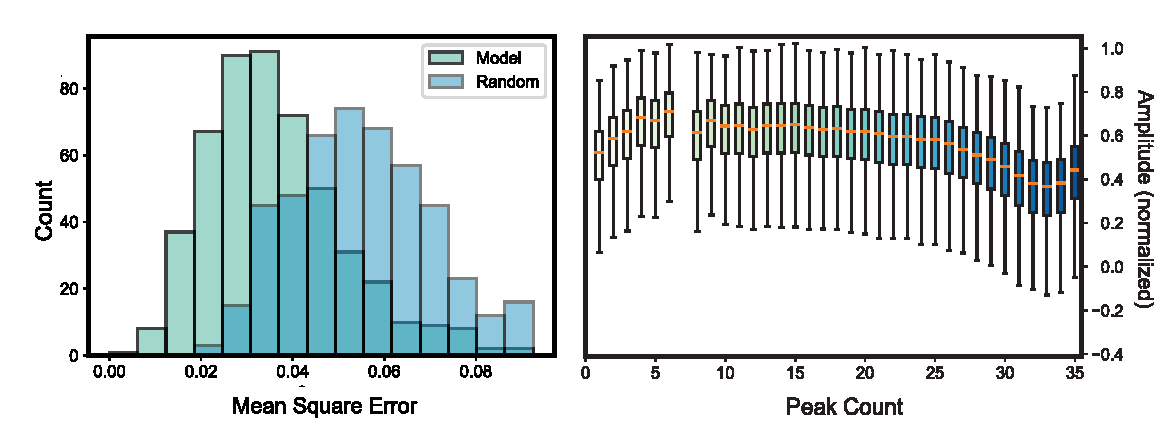
\includegraphics[width=6.5in]{figures/fig6a.eps}
		\caption{The left panel shows the mean square error histogram and verifies the model's predictive value while the right panel shows the wide array of possible values at each peak.}
\end{figure}

\noindent We can also plot the objective and ML-predicted waveforms along with the slots that generated them numerically for a couple of cases as in Figure 5 below.


\begin{figure}[H]
	\centering
	\subfloat{{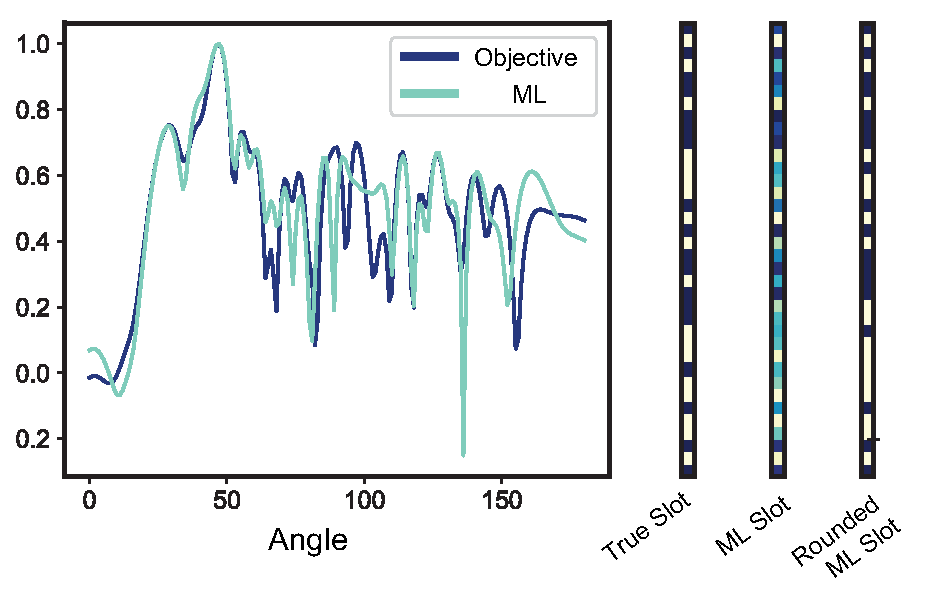
\includegraphics[height=2.1in]{figures/fig7_left_477.eps}}}
	\subfloat{{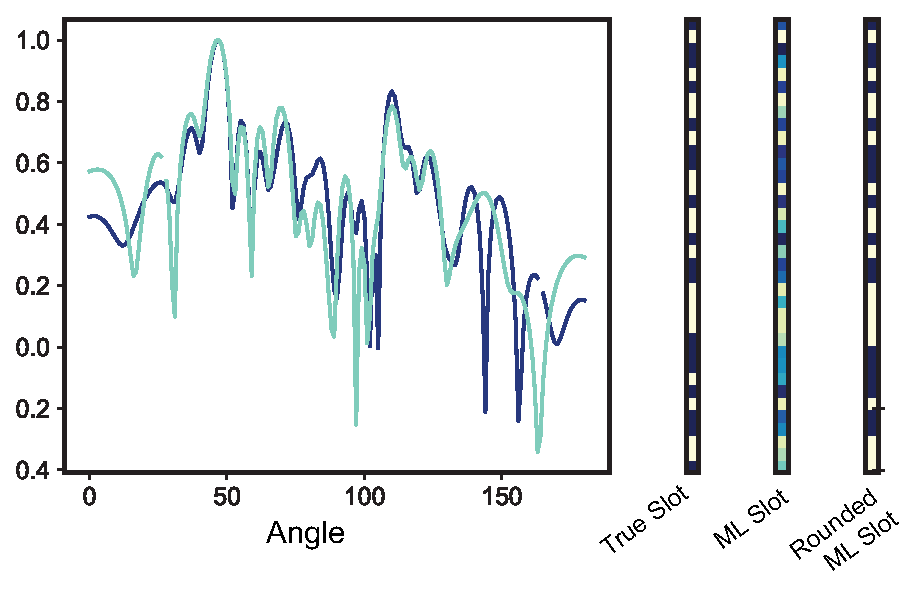
\includegraphics[height=2.1in]{figures/fig7_right_108.eps}}}
	\caption{Model predictions for two different peak profiles. The left-most slot design is the randomly generated slot used to generate this profile, the center plot shows the sigmoid probabilities of a transparent sub-slot, and the right-most plot shows the top 16 sub-slots from the probabilities. The MSEs of the left and right predictions are 0.0155 and 0.0250, respectively.}
\end{figure}

\noindent Overall, these examples showcase the ability of the model to produce reasonable slots that approximate the desired far-field signal. These two cases showcase the best performance of the model, but even with substantially higher values of mean-square error, the overall peak behavior is often well-preserved, albeit with less exact results and more missed peaks.  \\

\noindent We also wish to examine if our numerical predictions are present experimentally. First, using a terahertz time-domain spectroscopy (TDS), we measure and plot angle versus frequency for two different slots, one with a uniform periodic slot and one with our unique periodically-modulated slots as in Figure 6 below.

\begin{figure}[H]
	\centering
	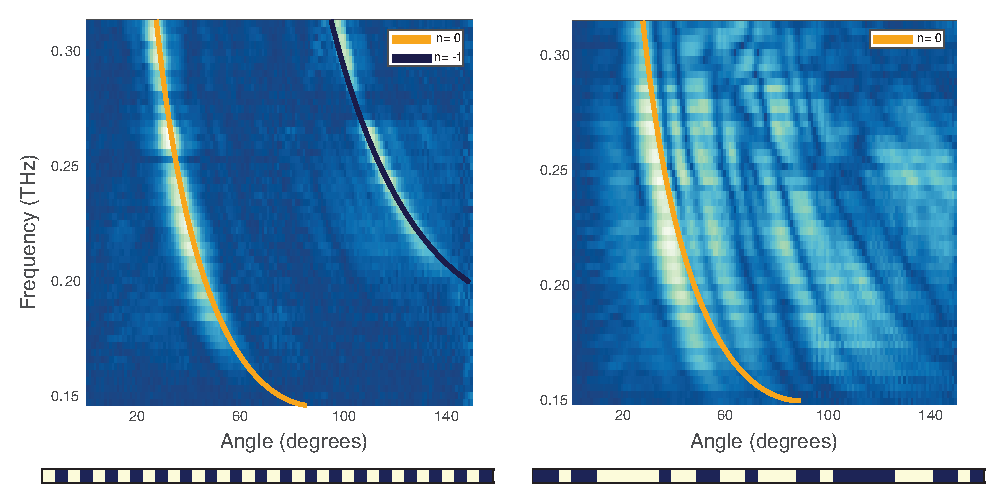
\includegraphics{figures/exp-fig1.eps}
	\caption{Experimental time-domain spectroscopy (TDS) measurements for two different slot designs, the left with only one periodicity and the right with a linear combination of periodicities.}
\end{figure}

\noindent Generally speaking, we observe what we expect from Floquet theory. For the simple periodic slot, we see the main, non-periodic mode in addition to the one fast-wave Floquet mode. However, at right, we see many Floquet modes at play due to the periodicially-modulated nature of the slot; these two plots pose a sharp contrast to one another and show how our method is capable of producing a multitude of possible slot designs. From the TDS data, we can extract the far-field signal at 200 GHz and plot against the simulation data (note this is different data than Figure 5).

\begin{figure}[H]
	\centering
	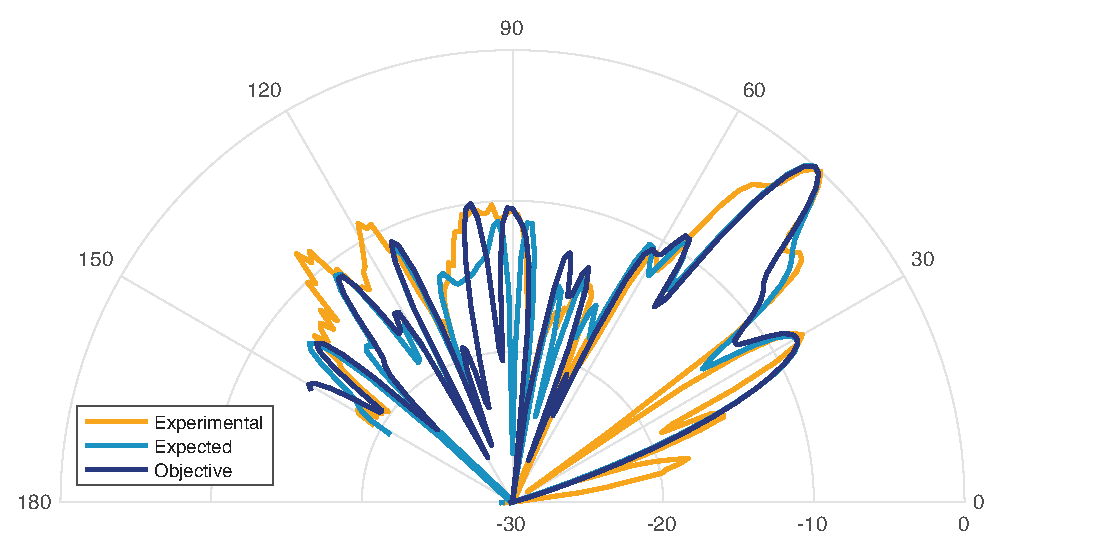
\includegraphics[height=2in]{figures/477exp.eps}
	\caption{Polar plots of experimental versus simulation data for both the objective and predicted slot; overall, the plots indicate excellent agreement, particularly at the peaks of highest magnitude.}
\end{figure}

\noindent We draw two primary conclusions from Figure 7, which are generated from the model's predictions for low values of MSE. First, the slot predicted by the model predicts a far-field signal quite similar to the objective function. Secondly, the experimental data generally agrees with the simulation data, particularly near the largest peaks, there are certainly differences between the numerical and experimental values. One possible cause is due to the relatively simple setup we are using to measure experimental data and the resulting geometrical difficulties of picking up back-scattering. However, the experimental measurements certainly serve as a proof of concept for further exploration.

\subsection*{Grey Sub-Slot Scheme}

\noindent This second scheme significantly expands the scope of the problem because each sub-slot can take one of five values instead of just two: fully metallic, 25\% transparent, 50\% transparent, 75\% transparent, and 100\% transparent. We again generate approximately 20,000 samples using numerical simulation where each sub-slot can take on these values using a transition boundary layer. This significantly increases the number of degrees of freedom within the model, as we see in the right panel of Figure 8 below; the range of values at each peak is broader than is seen than in Figure 4.

\begin{figure}[H]
	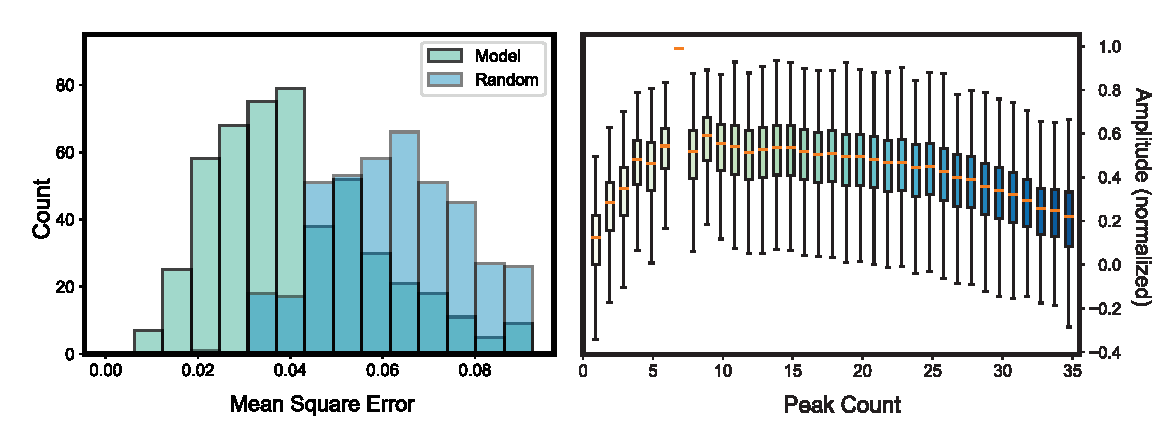
\includegraphics[width=6.5in]{figures/histboxgrey.eps}
		\caption{The left panel shows the mean square error histogram and verifies the model's predictive value while the right panel shows the wide array of possible values at each peak.}
\end{figure}

\noindent The left panel of Figure 8 shows the mean square error histogram for the 500 sets of testing data for which we numerically solved for the predicted slot's far-field pattern in order to compare its similarity to the objective. While the model performs similarly to the binary case (except for a slightly longer tail here), the control MSE histogram broadens and moves to the right. This means that our model performs better relative to the control with the greyscale scheme compared to the binary scheme, which is not unexpected given the increased degrees of freedom at play and the strength of neural network models at uncovering complex non-linear relationships.  \\


\noindent Like before in Figure 5, we can plot some of the model-generated slots and the resulting far-field patterns in order to get an idea of what sort of slots the model is producing, which we plot in Figure 9 below. Overall, we see close agreement between the objective and ML-predicted slots, particularly at the largest peaks and the overall profile of the wave.

\begin{figure}[H]
	\centering
	\subfloat{{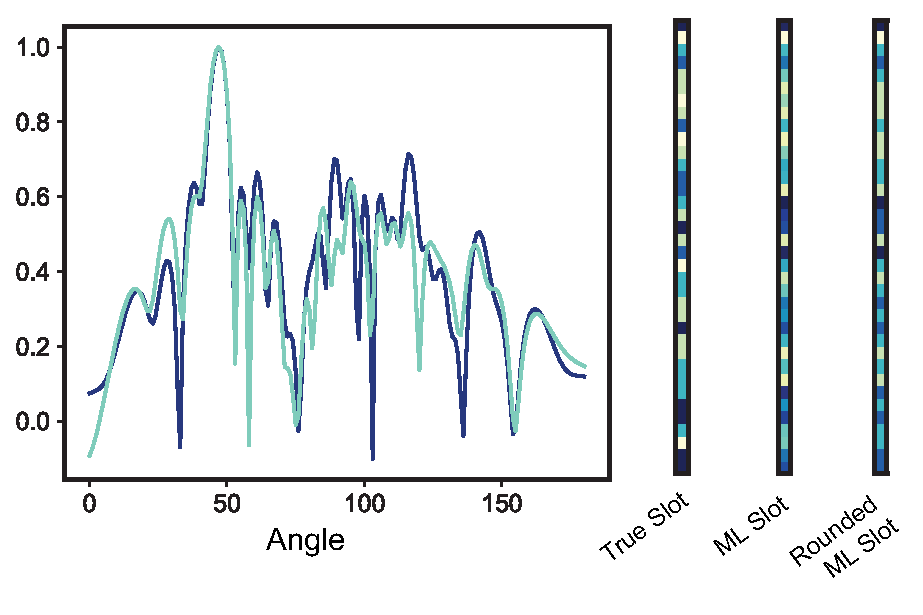
\includegraphics[height=2.1in]{figures/grey_example_71.eps}}}
	\subfloat{{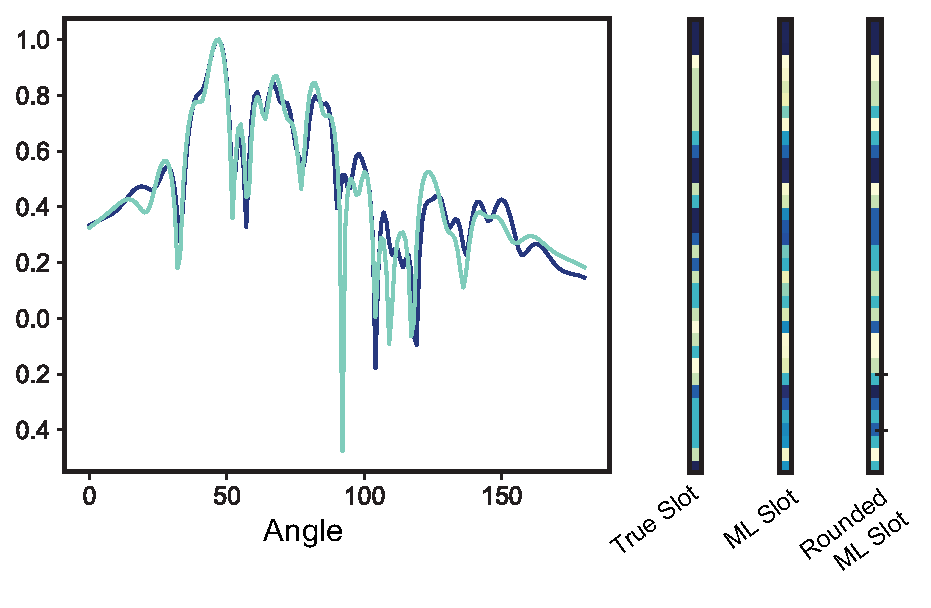
\includegraphics[height=2.1in]{figures/grey_example_127.eps}}}
	\caption{Model predictions for two different peak profiles using the greyscale scheme. The left slot design is the randomly generated greyscale slot used to generate the objective, the center plot shows the ideal transparency of each sub-slot, and the right plot shows those rounded into the buckets used in the simulation. The MSEs of the left and right predictions are 0.0127 and 0.0113.}
\end{figure}

\noindent As before, we are interested in comparing the results of our model and numerical simulations to experimental data. However, this is slightly more complicated experimental method -- we need to actually experimentally generate semi-transparent slots. We do this by using the aforementioned hot-stamping technique but instead of using black ink for metallic slots and the absence of ink for transparent slots, we calibrate our TDS system using ``grey'' slots, the idea being that changing the ink color within the greyscale spectrum will directly correlate with the amount of metal deposited on the surface of the antenna. We first calibrate shades of grey with transmission values, then using the shades of grey that conform to 25\%, 50\%, and 75\% transparency, we produce our LWAs using the exact same methodology as in the binary case.

\section*{Conclusion}

\bibliographystyle{plain}
\bibliography{references.bib}
\end{document}
